\chapter{Data Analysis} \label{ch:analysis}
This thesis details the method of transverse energy analysis through the use of $p_{T}$ spectra from the STAR BES data. As described in section \ref{subsec:tracking_STAR}, the TPCs and TOF detectors in STAR can identify particles as well as their trajectories and ultimately measure their multiplicity distributions with respect to the momenta. The available distributions were extrapolated to calculate the transverse energies and charged particle multiplicities. Details follow.

\section{STAR $p_{T}$ Spectra}
\citet{PhysRevC.96.044904} reports the results for the midrapidity ($\left|{y}\right| < 0.1$) $p_{T}$ spectra for six different identified hadrons, $\pi^+$, $\pi^-$, $K^+$, $K^-$, $p$, and $\bar{p}$, from the STAR experiment. The spectra come from $\sqrt{s_{NN}}$ = 7.7, 11.5, and 39 GeV Au+Au collisions data taken in the year 2010, and from $\sqrt{s_{NN}}$ = 19.6 and 27 GeV Au+Au collisions data taken in 2011, both as part of the BES Program. Figure \ref{fig:BESPaper_pTSpectra} \cite{PhysRevC.96.044904} shows the spectra corresponding to 39 GeV collisions categorized into seven different collision centralitiy classes. Additionaly, preliminary spectra were available from the STAR experiment for idenfitied lambdas and anti-lambdas \cite{YePrivateCommunication}. All of these spectra were used to calculate the total transverse energy per event per particle species. This result was then used to estimate the total transverse energy due to all the collision products. The corrections applied by \citet{PhysRevC.96.044904} to the raw data to obtain the spectra and the reported systematic uncertainties in their results are discussed below.
\begin{figure}[h]
  \centering
  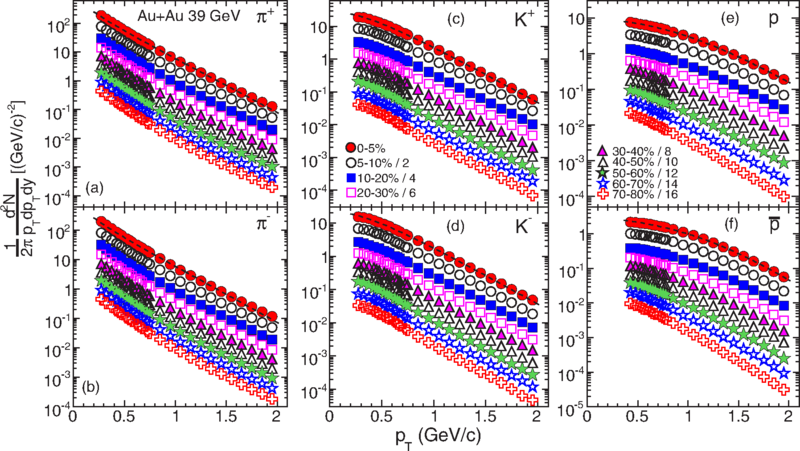
\includegraphics[width=6.5in]{../figures/PhysRevC-96-044904_pTSpectra_39.png}\\
  \caption{Transverse momentum spectra for $\pi^{+}$, $\pi^{-}$, $K^+$, $K^{-}$, $p$, and $\bar{p}$ at midrapidity ($|y|$ $<$ 0.1) from 39 GeV Au+Au collisions at RHIC. The fitting curves on the 0-5\% central collision spectra for pions, kaons, and protons/anti-protons represent, respectively, the Bose-Einstein, $m_{T}$-exponential, and double-exponential functions \cite{PhysRevC.96.044904}.}\label{fig:BESPaper_pTSpectra}
\end{figure}

\subsection{Corrections and Systematic Uncertainties}
Detector acceptance and efficiency of reconstructing particle tracks account for most of the correction applied to the raw spectra. The efficiency $\times$ acceptance correction factor is obtained as the ratio of the distribution of the reconstructed tracks from the experiment and the tracks simulated using the GEANT model of STAR. The inverse of this factor is used to scale the raw spectra. Figure \ref{fig:AdamczykCorrection1} shows typical efficiency $\times$ acceptance factors as functions of $p_{T}$ for 0-5\% central 7.7 GeV collisions.

Not all tracks formed in the TPC propagate to the TOF. A correction, called the TOF matching efficiency, is applied to the spectra obtained from the TOF. This correction is defined as the ratio of the number of tracks obtained from the TOF to the total number of tracks obtained from the TPC within the same acceptance. The inverse of the TOF matching efficiency is used to scale the TOF raw yields.

The algorithm used by STAR for track reconstruction assumes that each particle is a pion. A third correction is applied using a Monte Carlo simulation to account for the presence of the proton and the kaon tracks apart from the pion tracks. Two other corrections are obtained to subtract the backgrounds of secondary pions and protons produced from the interactions with the detector materials and those of the pions attributable to muon contamination and feed-down contribution from weak decays.

The systematic uncertainties are obtained by varying the analysis cuts and by estimating the tracking efficiencies for each of the identified particles. The former source contributes 4\%, 3\%, and 6\% respectively and the latter 5\% each for pions, kaons, and protons. Furthermore, the aforementioned energy loss correction contributes 3\% and 5\% systematic uncertainties for kaons and protons, respectively.

\begin{figure}[h]
  \centering
  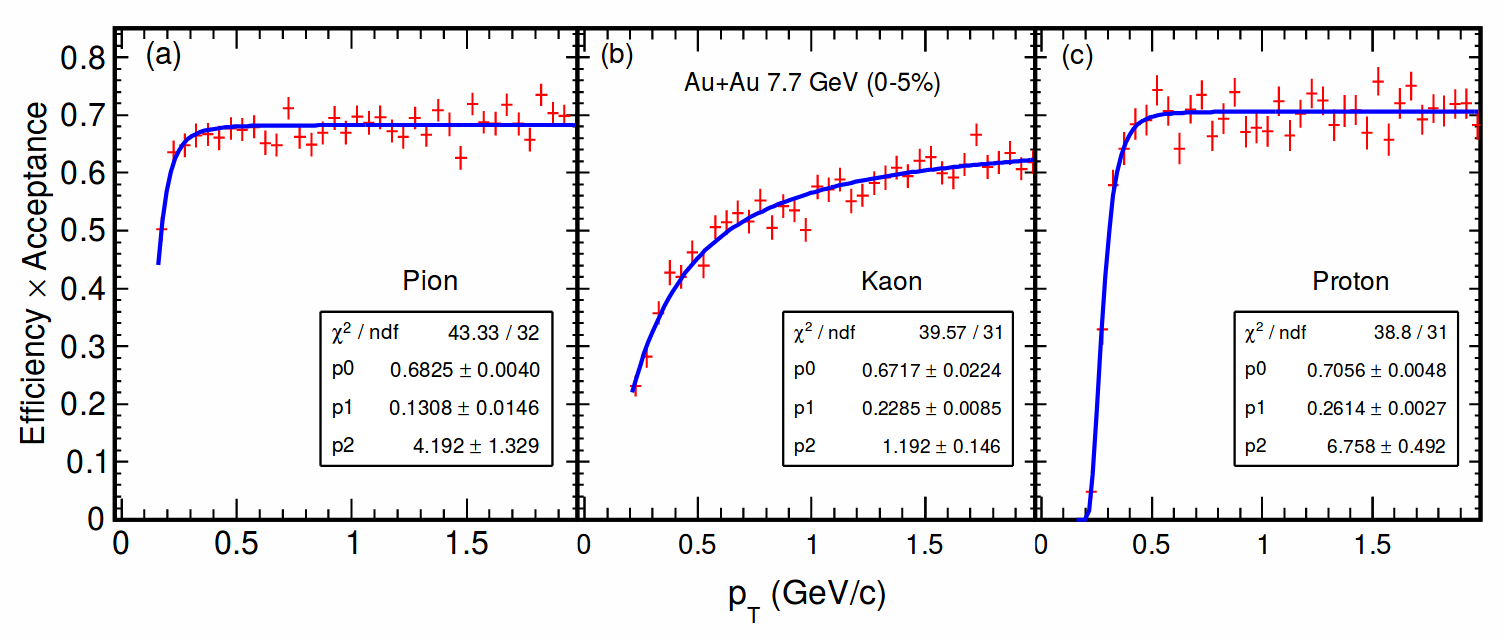
\includegraphics[width=6.5in]{../figures/Adamzyck_correction1.png}\\
  \caption{Midrapidity efficiency $\times$ acceptance as a function of $p_{T}$ calculated from STAR TPC Monte Carlo simulation of reconstructing (a) pions, (b) kaons, and (c) protons for 0-5\% central 7.7 GeV Au+Au collisions. The curves represent functional fits of the form $y \propto e^{-\frac{1}{x}}$ \cite{PhysRevC.96.044904}.}\label{fig:AdamczykCorrection1}
\end{figure}

\section{Extrapolation of Spectra}
The available spectra were limited to a range of transverse momenta from around 0.25 GeV/c to around 2 GeV/c (for pions). At higher momenta, with model-dependent values, the $p_{T}$ spectra may be dominated by hard-scattering processes. To account for the transverse energy corresponding to the momenta for which there were no available data, an extrapolation had to be used. The model used for the extrapolation and the associated statistics are discussed below.

\subsection{Boltzmann-Gibbs Blast Wave}
% https://arxiv.org/pdf/0812.1609.pdf
% https://arxiv.org/pdf/1703.02416.pdf
% 
The blast wave is a common model used in the analysis of particle momentum distributions \cite{Tang:2008ud,Tripathy:2017kwb,PhysRevC.96.044904}. The specific model used in this thesis is the Boltzmann-Gibbs blast wave (BGBW). This model assumes local thermal equilibrium at the kinetic freeze-out temperature for the applicability of a Boltzmann distribution. It also assumes a radially increasing velocity that attains a maximum value at the surface of the expanding fireball \cite{Tripathy:2017kwb}. The BGBW is represented by the equation: %It has the parameters mass, temperature, beta, v, and n. % Eq. 3.2 pg 52 from the analysis note

	\begin{equation}\label{eqn:BGBW}
	\frac{dN}{dp_{T}} \approx \int_{0}^{R} rdrp_{T}m_{T}I_{0}(\frac{p_{T}\sinh\rho}{T})K_{1}(\frac{m_{T}\cosh\rho}{T}),
	\end{equation}
where $\rho = \tanh^{-1}\beta$ is the flow profile, $\beta = \beta_{max}(\frac{r}{R})^{n}$ is the flow velocity, $n$ is the flow velocity profile exponent, $r$ is the radial distance from the collision vertex, $R$ is the distance of the expanding medium surface from the collision vertex, $m_{T}$ is the transverse mass given by Eq. \ref{eqn:mT}, $T$ is the thermal freeze-out temperature, and $I_{0}(x)$ and $K_{1}(x)$ ($x$ being the placeholder for the function arguments) are the modified Bessel functions of the first and second kind.

% I assume that any anomalies in the magnitude of the normalization parameter do not affect the results significantly insomuch as they don't lead to: (a) unreasonable relative errors in the extrapolated values of the transverse energy, (b) any of the spectral fits having the extrapolated transverse energy more than that calculated from just the available spectra, and (c) for the 200 GeV collision samples, at least, the extrapolation at higher $p_{T}$ being more than that at lower $p_{T}$.


\subsection{Fitting Spectra to BGBW}
Figure \ref{fig:fit} presents an example of a BGBW fit on one of the individual particle spectra with $\chi^{2}$/ndf as well as other statistics and the associated uncertainties. While this fit function is motivated by the Blast Wave model, the main goal of the fits is to extrapolate the data above and below the range where data are available. As long as the fit describes the data and the fraction of ET from the extrapolation is small compared to the ET calculated where there are data, the sensitivity of the results to the functional form of the fit is minimal. The fitting is done in the ROOT software framework which is widely used in high energy physics data analysis. $T$, $\beta$, and $n$ are treated as free parameters, while $m$ is fixed. The results of the fits for each of the spectra are tabulated in appendix \ref{app:fitResults}. 
%A parallel-coordinates plot is presented in the next chapter in fig. \ref{fig:parallelCoord}, which shows the measured centralities, two of the good-fit parameters, and the calculated transverse energies for 270 different particles (lambdas not included).

	\begin{figure}[h]
	  \centering
	  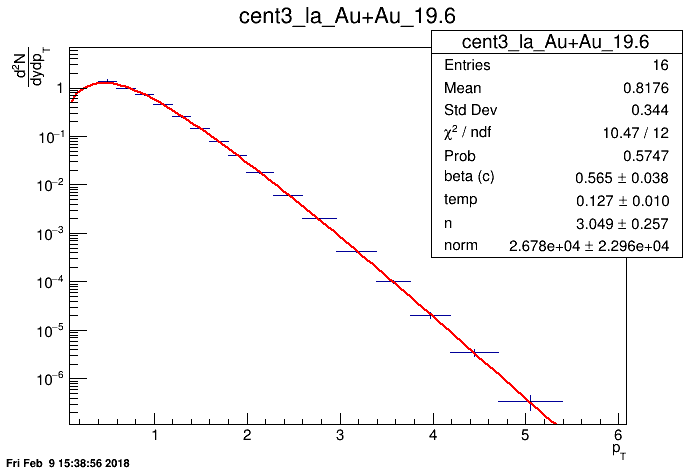
\includegraphics[width=6.5in]{figures/cent3_la_Au+Au_196.png}
	  \caption{Red curve shows the Boltzmann-Gibbs blast wave functional fit on the preliminary transverse momentum spectrum for lambda particles identified by the STAR detector for 19.6 GeV Au+Au collisions (10-15\% central). Parameters extracted from the chi-square goodness-of-fit test, as well as other statistics, are shown in the box on the top right.}\label{fig:fit}
	\end{figure}

%%%%%%%%%%%%%%%%%%%%%%%%%%%%%%%%%%%%%%%%%%%%%%%%%%%%%%%%%%%%%%%%%%%%%%%%%%%%%%
\section{Calculations from the Spectra}

\subsection{Calculation of $\frac{dE_{T}}{dy}$, $\frac{dE_{T}}{d\eta}$, $\frac{dN_{ch}}{dy}$, and $\frac{dN_{ch}}{d\eta}$}
The available multiplicity distribution for the $p_{T}$ range, $p_{T,low}$ to $p_{T,high}$, of a spectrum divided the total spectrum into three different regions: $(i)$ region where the experimental data are available, i.e., $p_{T,low}$ to $p_{T,high}$, $(ii)$ extrapolation region from $p_{T}$ = 0 GeV/c to $p_{T}$ = $p_{T,low}$, and $(iii)$ extrapolation region from $p_{T}$ = $p_{T,high}$ to $p_{T}$ = 10 GeV/c. Following the methods and the Jacobian transformation described in section \ref{section:calcFromSpectra}, $\frac{dE_{T}}{dy}$, $\frac{dE_{T}}{d\eta}$, $\frac{dN_{ch}}{dy}$, and $\frac{dN_{ch}}{d\eta}$ from the spectra were calculated by adding said quantities corresponding to the three different regions in the distribution.

\subsection{Assumptions, Estimation of Total $E_{T}$, and Uncertainties}\label{totalET}
It is assumed that most of the $E_{T}$ is attributable to the contributions from pions, kaons, protons, neutrons, lambdas, and their anti-particles. Contributions from heavier particles are assumed to be negligible, and there are some particles which are light but decay very rapidly into $\pi/K/p$ which are included in the spectra. It is also reasonable to assume that, at high energies, there should be roughly the same multiplicity of all the isospin states and anti-particles of a final state particle. This assumption was partially tested by comparing the $E_{T}$ values calculated for the identified charged particles with those independently calculated for their anti-particles for the same values of collision energy and centrality. The comparisons revealed the $E_{T}$ values of the particles being almost exactly equal to those of the anti-particles. This assumption is used to account for the energies of the isospin states of the pions, kaons and protons that were not identified.

Table \ref{table:isospinStates} lists the isospin states and the anti-particles associated with the pion, the kaon, the proton, and the lambda particles.
	\begin{table}[h!]
	\centering
	\begin{tabular}{|c c|}
	%\tabletypesize{\scriptsize}
	%\rotate
	\hline
	Particle & Isospin multiplets \\ [0.5ex]
	\hline
	\hline
	pion & $\pi^{+}, \pi^{0}, \pi^{-} $ \\
	kaon & $K^{+}, K^{0}, K^{-}, \bar{K}^{0}$ \\
	proton & $p, n, \bar{p}, \bar{n}$  \\
	lambda & $\Lambda, \bar{\Lambda}$  \\ [1ex]
	\hline
	\end{tabular}
	\caption{Isospin states of different identified particles.}
	\label{table:isospinStates}
	\end{table}
	
The total $E_{T}$ for all the particles would then be:	
	\begin{equation}\label{eqn:TotET}
	E_{T} = \frac{3}{2}(E_{T}^{\pi^{+}}+E_{T}^{\pi^{-}}) + 2(E_{T}^{K^{+}}+E_{T}^{K^{-}}) + 2(E_{T}^{p}+E_{T}^{\bar{p}}) + E_{T}^{\Lambda} + E_{T}^{\bar{\Lambda}}
	\end{equation}
	
There are three major sources of systematic uncertainties: $(i)$ uncertainties in the spectra available from \cite{PhysRevC.96.044904}, $(ii)$ assumptions involved in the fitting function which mainly affects the extrapolation toward lower $p_{T}$ values, and $(iii)$ assumption regarding particle ratios and that most of the $E_{T}$ is only carried by the particles listed in table \ref{table:isospinStates}. Uncertainties from the first source are propagated in the parameter uncertainties in the best-fit function, which are then propagated using the covariance matrices of the parameters to the $E_{T}$ and $N_{ch}$ results. Statistical uncertainties in the available data, which were small as compared to the corresponding systematic uncertainties, were added to the systematic uncertainties in quadrature. Uncertainties from the second source can be calculated by using several models, apart from the BGBW, to perform the extrapolations. Each of the models would have different assumptions involved in it, and the variation in the $E_{T}$ results from the different models can give an estimate of the systematic uncertainties arising from the difference in the assumptions. Calculation of these uncertainties are left for future work. Uncertainties from the third source result from the assumption of the calculation and are not quantified. The uncertainties are assumed to be 100\% correlated point to point and uncorrelated between different particles.
 
\subsection{Lambda Centrality Adjustments and $E_{T}$ Interpolations}
The centrality bins corresponding to the lambda spectra were slightly different from those corresponding to the rest of the particles. The centralities were binned the same way from 0\% to 40\%. However, the peripheral centralities for the lambdas were binned into 40-60\% and 60-80\% bins, whereas, for the rest of the particles, the peripheral centralities were binned into 40-50\%, 50-60\%, 60-70\%, and 70-80\% bins. For consistency, the lambdas $E_{T}$ calculations were interpolated to the centralities corresponding to $\pi/K/p$ using the $Eval()$ method of the $TGraph$ class in the ROOT framework. Specifically, a cubic spline was used to interpolate $E_{T}/0.5N_{part}$ as a function of $N_{part}$ because the former was known from past experiments to not fluctuate significantly as a function of the latter. The relative uncertainty corresponding to the adjacent data point with the higher relative uncertainty was used as the relative uncertainty for the interpolated data point.
